\documentclass[tikz, border=10pt]{standalone}
\usepackage{pgfplots}
\pgfplotsset{compat=1.18}

\begin{document}
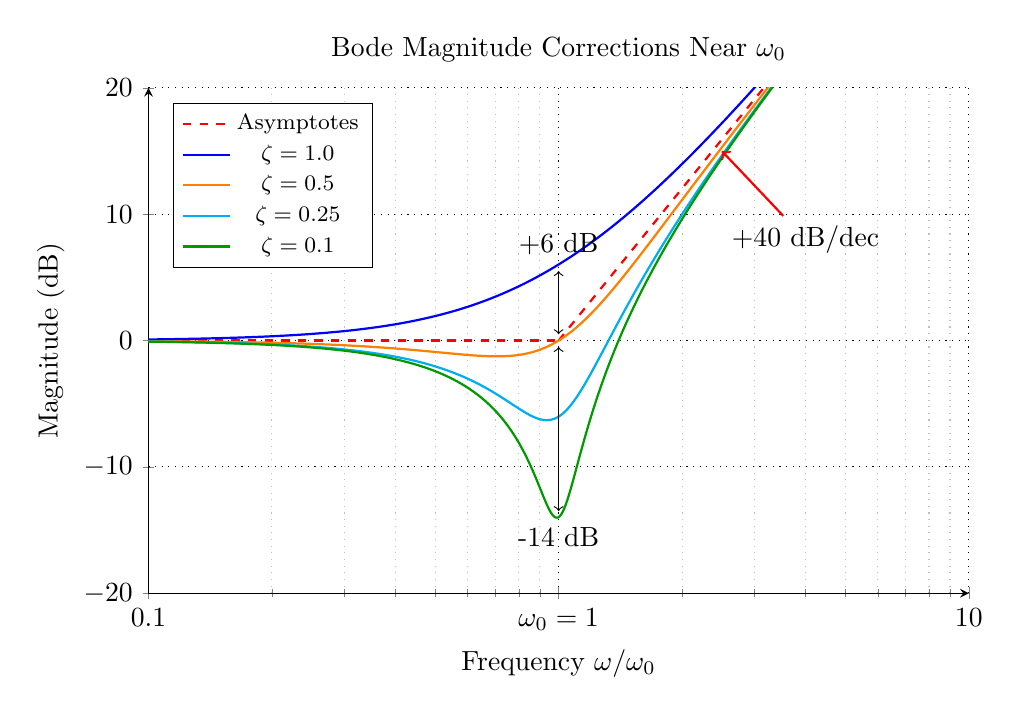
\begin{tikzpicture}
    \begin{semilogxaxis}[
        width=12cm, height=8cm,
        xlabel={Frequency $\omega/\omega_0$},
        ylabel={Magnitude (dB)},
        xmin=0.1, xmax=10,
        ymin=-20, ymax=20,
        grid=both,
        major grid style={dotted, black},
        minor grid style={dotted, gray!50},
        axis lines=left,
        xtick={0.1, 1, 10},
        xticklabels={$0.1$, $\omega_0=1$, $10$},
        legend pos=north west,
        legend style={font=\footnotesize},
        title={Bode Magnitude Corrections Near $\omega_0$}
    ]

    % Asymptotes
    % Use forget plot for the first segment so it doesn't consume a legend entry
    \addplot[thick, red, dashed, domain=0.1:1, forget plot] {0};
    \addplot[thick, red, dashed, domain=1:10] {40*log10(x)};
    \addlegendentry{Asymptotes}

    % Zeta = 1.0 (+6dB at corner)
    \addplot[thick, blue, domain=0.1:10, samples=200] {20*log10(1 + x^2)};
    \addlegendentry{$\zeta = 1.0$}

    % Zeta = 0.5 (0dB at corner)
    \addplot[thick, orange, domain=0.1:10, samples=200] {10*log10((1 - x^2)^2 + (x)^2)};
    \addlegendentry{$\zeta = 0.5$}

    % Zeta = 0.25 (-6dB at corner)
    \addplot[thick, cyan, domain=0.1:10, samples=300] {10*log10((1 - x^2)^2 + (0.5*x)^2)};
    \addlegendentry{$\zeta = 0.25$}

    % Zeta = 0.1 (-14dB at corner)
    \addplot[thick, green!60!black, domain=0.1:10, samples=500] {10*log10((1 - x^2)^2 + (0.2*x)^2)};
    \addlegendentry{$\zeta = 0.1$}

    % Annotations
    \node[anchor=south] at (axis cs: 1, 6) {+6 dB};
    \node[anchor=north] at (axis cs: 1, -14) {-14 dB};
    
    % Slope annotation
    \node (slope_label) at (axis cs: 4, 8) {+40 dB/dec};
    \draw[->, thick, red] (slope_label) -- (axis cs: 2.5, 15);
    
    % Arrows
    \draw[<->] (axis cs: 1, 0.5) -- (axis cs: 1, 5.5);
    \draw[<->] (axis cs: 1, -0.5) -- (axis cs: 1, -13.5);

    \end{semilogxaxis}
\end{tikzpicture}
\end{document}
